% This file was created with tikzplotlib v0.10.1.post9.
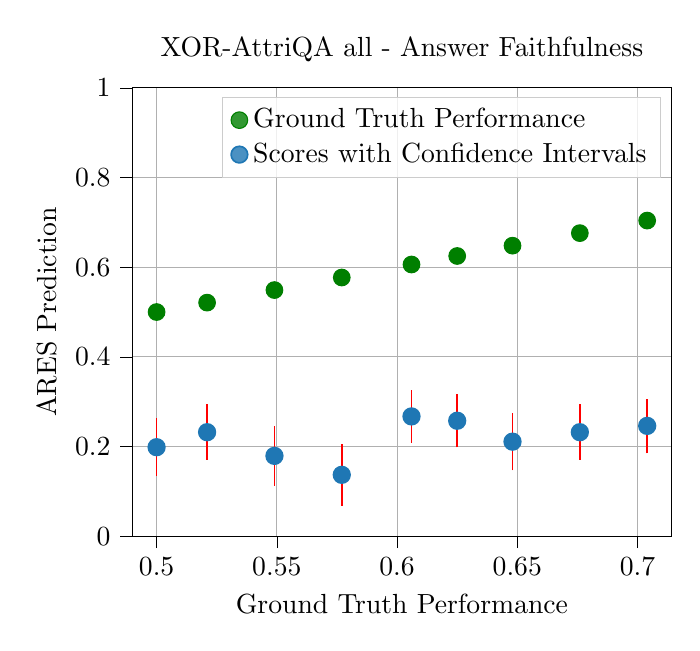
\begin{tikzpicture}

\definecolor{darkgrey176}{RGB}{176,176,176}
\definecolor{green01270}{RGB}{0,127,0}
\definecolor{lightgrey204}{RGB}{204,204,204}
\definecolor{steelblue31119180}{RGB}{31,119,180}

\begin{axis}[
legend cell align={left},
legend style={
  fill opacity=0.8,
  draw opacity=1,
  text opacity=1,
  draw=lightgrey204,
  mark options={mark size=3}
},
tick align=outside,
tick pos=left,
title={XOR-AttriQA all - Answer Faithfulness},
x grid style={darkgrey176},
xlabel={Ground Truth Performance},
xmajorgrids,
xmin=0.4898, xmax=0.7142,
xtick style={color=black},
y grid style={darkgrey176},
ylabel={ARES Prediction},
ymajorgrids,
ymin=0, ymax=1,
ytick style={color=black}
]
\addplot [draw=green01270, fill=green01270, mark size=3pt, mark=*, only marks]
table{%
x  y
0.5 0.5
0.521 0.521
0.549 0.549
0.577 0.577
0.606 0.606
0.625 0.625
0.648 0.648
0.676 0.676
0.704 0.704
};
\addlegendentry{Ground Truth Performance}
\path [draw=red, semithick]
(axis cs:0.5,0.134)
--(axis cs:0.5,0.263);

\path [draw=red, semithick]
(axis cs:0.521,0.17)
--(axis cs:0.521,0.294);

\path [draw=red, semithick]
(axis cs:0.549,0.113)
--(axis cs:0.549,0.246);

\path [draw=red, semithick]
(axis cs:0.577,0.068)
--(axis cs:0.577,0.206);

\path [draw=red, semithick]
(axis cs:0.606,0.208)
--(axis cs:0.606,0.326);

\path [draw=red, semithick]
(axis cs:0.625,0.198)
--(axis cs:0.625,0.317);

\path [draw=red, semithick]
(axis cs:0.648,0.147)
--(axis cs:0.648,0.275);

\path [draw=red, semithick]
(axis cs:0.676,0.17)
--(axis cs:0.676,0.294);

\path [draw=red, semithick]
(axis cs:0.704,0.185)
--(axis cs:0.704,0.307);

\addplot [semithick, steelblue31119180, mark=*, mark size=3, mark options={solid}, only marks]
table {%
0.5 0.198472222222222
0.521 0.231971830985915
0.549 0.179154929577465
0.577 0.136901408450704
0.606 0.267183098591549
0.625 0.2575
0.648 0.210845070422535
0.676 0.231971830985915
0.704 0.246056338028169
};
\addlegendentry{Scores with Confidence Intervals}
\end{axis}

\end{tikzpicture}
